\documentclass{beamer}

\usepackage[utf8]{inputenc} % Encoding
\usepackage{graphicx} % Work with graphics
\usepackage{ragged2e} % Introduce justified text
\usepackage{braket} % Dirac's braket notation
\usepackage{xcolor} % Colors
\usepackage{bm} % Bold symbols in equations
\usepackage[export]{adjustbox} % Add color to edges of figure
\usepackage[ruled,vlined]{algorithm2e} % Support for algorithms
\usepackage{listings} % Support for code snippets
\usepackage{caption}  % Use subfigures
\usepackage{subcaption} % Use subfigures
\usepackage{verbatim}

\usetheme{Warsaw}

% Required for including image in text

\newcommand*{\img}[1]{
    \raisebox{-.15\baselineskip}{
        \includegraphics[
        height=\baselineskip,
        width=3\baselineskip,
        keepaspectratio,
        ]{#1}
    }
}

% Create macro for norm

\newcommand{\norm}[1]{\left\lVert#1\right\rVert}

% Macro to add page number

\newcommand*\oldmacro{}%
\let\oldmacro\insertshorttitle%
\renewcommand*\insertshorttitle{%
   \oldmacro\hfill%
   \insertframenumber\,/\,\inserttotalframenumber}

% Figures directory

\graphicspath{{./Figures/}}

% Title page information

\title[Intro MCTDH]{A \emph{gentle} introduction to MCTDH}
%\subtitle{\footnotesize With emphasis in potential representations}
\author[Panadés-Barrueta]{Ramón L. Panadés-Barrueta}
\institute{Computational Chemical Physics Group. \\ University of Twente.}
\date{\small November 5, 2020}
\titlegraphic{\includegraphics[width=1.65cm]{trex_logo.png}\hspace*{7.00cm}~%
   \includegraphics[width=2cm]{ut_logo.pdf}}

% ToC in each section

\AtBeginSection[]
{
  \begin{frame}
    \tableofcontents[currentsection]
  \end{frame}
}

% Presentation's content

\begin{document}

\frame{\titlepage}

% Initial table of contents
\begin{frame}
  \tableofcontents
\end{frame}

\section{Nuclear Quantum Dynamics}\label{nqd}

\begin{frame}
  \frametitle{Nuclear Quantum Dynamics}
  \begin{block}{What}
   \justifying{}
   The subfield of Theoretical Chemistry in which both the \textbf{electrons} and the \textbf{nuclei} of
   a molecular system are treated in a \textbf{quantum-mechanical} manner. 
  \end{block}
  \begin{exampleblock}{When}<2->
    \begin{itemize}
    \item Spectroscopy (e.g. IR transitions)
    \item Quantum tunneling
    \item Vibronic coupling
    \item ZPE determination
    \end{itemize}
  \end{exampleblock}
\end{frame}

\begin{frame}
  \frametitle{Nuclear Quantum Dynamics}
  Find the numerical solution of the TDSE truncating the Hilbert space to a finite dimension (Galerkin's method):
\begin{equation}
  i\hbar\frac{\partial\Psi}{\partial t} = \hat{H}\Psi
\end{equation}
Given a parametric representation of the WF (\(\Psi\)), the optimal solution can be found using the Dirac-Frenkel Variational Principle (DF-VP):
\begin{equation}
	\braket{\delta\Psi|\hat{H}-i\frac{\partial }{\partial t}|\Psi} = 0
\end{equation}
\end{frame}

\subsection{The Standard method}\label{stdmeth}

\begin{frame}
  \frametitle{The Standard method}
  Most direct representation of the WF\@: 
\begin{equation}
	\Psi(q_i,\ldots, q_f, t) = \sum_{j_1=1}^{N_1}\cdots\sum_{j_f=1}^{N_f} C_{j_1\ldots j_f}(t)\prod_{\kappa=1}^f\varphi^{(\kappa)}_{j_{\kappa}}(q_{\kappa})
	\label{stme}
\end{equation}
After plugging this WF into the DF-VP, and performing the corresponding algebra we obtain
the following EOMs:
\begin{block}{}
\begin{align}
\begin{split}
	i\dot{C}_L &= \sum_J \braket{\varphi_L|\hat{H}|\varphi_J}C_J \\
	\bm{C}(t) &= e^{-i\bm{H}t}\bm{C}(0)
\end{split}
\end{align}
\end{block}
where we have introduced the composite indexes \(J = (j_1,\ldots,j_f)\).

\end{frame}

\subsection{The Time-Dependent Hartree method}\label{tdh}

\begin{frame}
  \frametitle{The Time-Dependent Hartree method}
  \justifying{}
  If we now consider time-dependent single-particle functions (SPFs):
\begin{equation}
  \Psi(q_1,\ldots, q_f, t) = A(t)\prod^f_{\kappa=1}\underbrace{
	\sum_{\mu=1}^{N_{\kappa}}c_{\mu}^{(\kappa, j_{\kappa})}(t)\cdot \chi^{(\kappa)}_{\mu}(q_{\kappa})}_{\varphi_{\kappa}(q_{\kappa}, t)}
\end{equation}
and use the DF-VP with arbitrary real constraints \(g_{\kappa} = i\braket{\varphi_{\kappa}(t)|\dot{\varphi}_{\kappa}(t)}\), we get the EOMs:

\begin{block}{}
  \begin{equation}
    \begin{split}
      A(t) &= A(0) \cdot e^{-i\int_0^t E(t')dt'} \\
      i\dot{\varphi}_{\kappa} &= (\mathcal{H}^{(\kappa)} - E)\varphi_{\kappa}
    \end{split}
  \end{equation}
\end{block}
with \(\mathcal{H}^{(\kappa)} = \braket{\Phi^{(\kappa)}|H|\Phi^{(\kappa)}}\).
\end{frame}

\begin{frame}
  \frametitle{Limitations of SM and TDH}
  \begin{exampleblock}{Standard method}
    \justifying{}
    Its application is largely limited due to the \textbf{curse of dimensionality}. Only systems up to four atoms (6D) can be addressed in practice.
  \end{exampleblock}
  \begin{block}{Time-Dependent Hartree}
    A better approach, but physically inaccurate. The \textbf{nuclear correlation} is harder to retrieve
    than the electronic correlation due to the nuclei's larger mass. The character of the nuclear WF is inherently \textbf{multiconfigurational}. 
  \end{block}
\end{frame}

\section{The Multiconfiguration Time-Dependent Hartree method}\label{mctdh}

\begin{frame}
  \frametitle{Ansätze comparison}
  \vspace{-.3cm}
  \begin{block}{Standard Method (CI)}
    \begin{equation}
      \Psi(q_i,\ldots, q_f, t) = \sum_{j_1=1}^{N_1}\cdots\sum_{j_f=1}^{N_f} C_{j_1\ldots j_f}(t)\prod_{\kappa=1}^f\varphi^{(\kappa)}_{j_{\kappa}}(q_{\kappa})
    \end{equation}
  \end{block}
  \begin{exampleblock}{Time-Dependent Hartree (HM)}<2->
    \begin{equation}
      \Psi(q_1,\ldots, q_f, t) = A(t)\prod^f_{\kappa=1}\varphi_{\kappa}^{(\kappa)}(q_{\kappa}, t)
    \end{equation}
  \end{exampleblock}

  \begin{alertblock}{Multiconfiguration Time-Dependent Hartree (MCSCF)}<3->
    \begin{equation}
      \Psi(q_1,\ldots, q_f, t) = \sum^{n_1}_{j_1=1}\cdots\sum^{n_f}_{j_f=1}A_{j_1,\ldots,j_f}(t)\prod^{f}_{\kappa=1}\varphi^{(\kappa)}_{j_{\kappa}}(q_{\kappa}, t)
      \label{mctdh_antz}
    \end{equation}
  \end{alertblock}
\end{frame}

\begin{frame} 
  \frametitle{MCTDH origins and distribution}
  \justifying{
  MCTDH was originally developed by Meyer and coworkers from the University of Heidelberg, in the early nineties\@:}
\begin{center}
  \includegraphics[scale=0.5, cfbox=blue 1pt]{first_mctdh.png}
\end{center}
There are currently three major implementations of the algorithm:
\begin{center}
  \includegraphics[scale=.07]{manthe.png}
  \hspace{.5cm}
  \includegraphics[scale=.07]{dieter.jpg}
  \hspace{.5cm}
\includegraphics[scale=.2]{graham.png}
\end{center}

  
\end{frame}

\subsection{EOMs}\label{eom}

\begin{frame}
  \frametitle{The MCTDH EOMs}
  The MCTDH ansatz has a very flexible Sum-of-Products (SOP) form:
    \begin{equation}
      \Psi(q_1,\ldots, q_f, t) = \sum^{n_1}_{j_1=1}\cdots\sum^{n_f}_{j_f=1}A_{j_1,\ldots,j_f}(t)\prod^{f}_{\kappa=1}\varphi^{(\kappa)}_{j_{\kappa}}(q_{\kappa}, t)
    \end{equation}
    with time dependent SPFs
    \begin{equation}
      \label{spf}
	\varphi^{(\kappa)}_{j_{\kappa}}(q_{\kappa}, t) = \sum_{\mu=1}^{N_{\kappa}}c_{\mu}^{(\kappa, j_{\kappa})}(t)\cdot \chi^{(\kappa)}_{\mu}(q_{\kappa})
    \end{equation}
  The \(\chi^{(\kappa)}_{\mu}(q_{\kappa})\) are typically DVR functions.
  
\end{frame}

\begin{frame}
  \frametitle{The MCTDH EOMs}
  \justifying{
  The \emph{ansatz} WF is determined up to a multiplicative constant. To derive the EOMs arbitrary constraint operators (\(\hat{g}^{(\kappa)}\)) are introduced:}
\begin{equation}
	i\braket{\varphi^{(\kappa)}_l|\dot{\varphi}^{(\kappa)}_j} = \braket{\varphi^{(\kappa)}_l|\hat{g}^{(\kappa)}|\varphi^{(\kappa)}_l}
\end{equation}
Using once again the DF-VP we get (for \(\hat{g}^{(\kappa)} \equiv 0\)):

\begin{block}{}
\begin{align}
\begin{split}
i\dot{A}_J &= \sum_L \braket{\Phi_J|\hat{H}|\Phi_L}A_L \\
i\dot{\varphi}^{(\kappa)}_j &= (1 - \hat{P}^{(\kappa)})\sum_{k,l=1}^{n_{\kappa}}(\bm{\rho}^{(\kappa)^{-1}})_{jk}\braket{\hat{H}}_{kl}^{(\kappa)}\varphi^{(\kappa)}_l
\label{mctdh_eom}
\end{split}	
\end{align}
\end{block}
      
\end{frame}

\begin{frame}
  \frametitle{The MCTDH EOMs}
 \vspace{-.3cm}
\begin{block}{}
\begin{align}
\begin{split}
i\dot{A}_J &= \sum_L \braket{\textcolor{red}{\Phi_J}|\hat{H}|\textcolor{red}{\Phi_L}}A_L \\
i\dot{\varphi}^{(\kappa)}_j &= (1 - \textcolor{blue}{\hat{P}^{(\kappa)}})\sum_{k,l=1}^{n_{\kappa}}(\textcolor{cyan}{{\bm{\rho}^{(\kappa)}}^{-1}})_{jk}\textcolor{magenta}{\braket{\hat{H}}_{kl}^{(\kappa)}}\varphi^{(\kappa)}_l
\label{mctdh_eom}
\end{split}	
\end{align}
\end{block}
 \vspace{-.35cm}
\begin{equation}
\textcolor{red}{\Phi_J = \prod_{\kappa=1}^f\varphi_{j_{\kappa}}^{(\kappa)}}
\end{equation}
\begin{equation}
\textcolor{cyan}{\rho_{kl}^{(\kappa)} = \braket{\Psi_k^{(\kappa)}|\Psi_l^{(\kappa)}}  = \sum_{J^{\kappa}}A_{J_{k}^{\kappa}}^*A_{J_{l}^{\kappa}}} \quad \textcolor{magenta}{\braket{\hat{H}}_{kl}^{(\kappa)} = \braket{\Psi_k^{(\kappa)}|\hat{H}|\Psi_l^{(\kappa)}}}
\end{equation}
\begin{equation}
	\textcolor{blue}{\hat{P}^{(\kappa)} = \sum_{j=1}^{n_{\kappa}}\ket{\varphi_j^{(\kappa)}}\bra{\varphi_j^{(\kappa)}}}
\end{equation}

\end{frame}

\begin{frame}
  \frametitle{MCTDH integration scheme}
  The MCTDH-EOMs solution is expensive due to the large amount of multidimensional integrals to solve. Since the \textbf{mean fields} are not strongly oscillating we can consider (CMF integration):
  \begin{block}{}
\begin{align}
\begin{split}
i\dot{A}_J &= \sum_L \bar{\mathcal{K}}_{JL}A_J \\
i\dot{\varphi}^{(1)}_j &= (1 - \hat{P}^{(1)})\{\hat{h}^{(1)}\varphi^{(1)}_j + \sum_{k,l=1}^{n_{1}}({\bm{\rho}^{(1)}}^{-1})_{jk}\braket{\bar{H}_R}_{kl}^{(1)}\varphi^{(1)}_l\} \\
           &\vdots \\
i\dot{\varphi}^{(f)}_j &= (1 - \hat{P}^{(f)})\{\hat{h}^{(f)}\varphi^{(f)}_j + \sum_{k,l=1}^{n_{f}}({\bm{\rho}^{(f)}}^{-1})_{jk}\braket{\bar{H}_R}_{kl}^{(f)}\varphi^{(f)}_l\}  
\label{mctdh_eom_mod_dec}
\end{split}	
\end{align}
\end{block}
  
\end{frame}
\begin{frame}
  \frametitle{Mode combination}
  Nothing prevents us from grouping physical coordinates into logical particles:
\begin{align}
\begin{split}
	Q_{\kappa} &\equiv (q_{\kappa,1}, q_{\kappa,1}, \ldots, q_{\kappa,d}) \\
	\varphi_{j}^{(\kappa)}(Q_{\kappa}, t) &= \varphi_{j}^{(\kappa)}(q_{\kappa,1}, q_{\kappa,1}, \ldots, q_{\kappa,d}, t)
\end{split}
\end{align}
Under these conditions, the MCTDH \emph{ansatz} will take the form:
\begin{align}
  \begin{split}
    \Psi(Q_1,\ldots, Q_p, t) &= \sum^{n_1}_{j_1=1}\cdots\sum^{n_p}_{j_p=1}A_{j_1,\ldots,j_p}(t)\prod^{p}_{\kappa=1}\varphi^{(\kappa)}_{j_{\kappa}}(Q_{\kappa}, t) \\
	\varphi_{j}^{(\kappa)}(Q_{\kappa}, t) &= \sum_{i_1 \ldots i_d} C^{(\kappa, j)}_{i_1 \ldots i_d}(t)\prod^{d}_{\nu=1}
	\chi^{(\kappa, \nu)}(q_{\kappa, \nu})
  \end{split}
	\label{mctdh_antz_mc}
\end{align}
  
\end{frame}

\begin{frame}
  \frametitle{Multilayer MCTDH (3-layer case)}
We can propagate the multidimensional SPFs with MCTDH itself!
\begin{equation}
	\Psi(q_1, q_2, q_3, t) = \sum_{j_{12}=1}^{n_{12}}\sum_{j_3 = 1}^{n_3}A_{j_{12}j_3}(t)\textcolor{red}{\varphi^{(12)}_{j_{12}}(q_1,q_2,t)}\varphi^{(3)}_{j_{3}}(q_3,t)
\end{equation}
where we have introduced:
\begin{equation}
	\textcolor{red}{\varphi^{(12)}_{j_{12}}(q_1,q_2,t) = \sum_{k_1 = 1}^{n_1}\sum_{k_2=1}^{n_2}B_{k_1,k_2}^{(12,j_{12})}\prod_{\mu=1}^2} \textcolor{blue}{\xi_{k_{\mu}}^{(\mu)}(q_{\mu},t)}
\end{equation}
and:
\begin{equation}
	\textcolor{blue}{\xi_{k_{\mu}}^{(\mu)}(q_{\mu},t) = \sum_{i_{\mu}=1}^{N_{\mu}} c_{i_{\mu}}^{(\mu,k_{\mu})}\chi_{i_{\mu}}^{(\mu)}(q_{\mu})}
\end{equation}
\end{frame}

\begin{frame}
  \frametitle{Multilayer MCTDH (3-layer case)}
  \begin{minipage}{0.3\linewidth}
    \tiny{
\begin{equation*}
	\Psi(q_1, q_2, q_3, t) = \sum_{j_{12}=1}^{n_{12}}\sum_{j_3 = 1}^{n_3}A_{j_{12}j_3}(t)\textcolor{red}{\varphi^{(12)}_{j_{12}}(q_1,q_2,t)}\varphi^{(3)}_{j_{3}}(q_3,t)
\end{equation*}
\begin{equation*}
	\textcolor{red}{\varphi^{(12)}_{j_{12}}(q_1,q_2,t) = \sum_{k_1 = 1}^{n_1}\sum_{k_2=1}^{n_2}B_{k_1,k_2}^{(12,j_{12})}\prod_{\mu=1}^2} \textcolor{blue}{\xi_{k_{\mu}}^{(\mu)}(q_{\mu},t)}
\end{equation*}
\begin{equation*}
	\textcolor{blue}{\xi_{k_{\mu}}^{(\mu)}(q_{\mu},t) = \sum_{i_{\mu}=1}^{N_{\mu}} c_{i_{\mu}}^{(\mu,k_{\mu})}\chi_{i_{\mu}}^{(\mu)}(q_{\mu})}
\end{equation*}}
\end{minipage}
\hfill
  \begin{minipage}{0.4\linewidth}
  \begin{center}
    \includegraphics[scale=.26]{mlmctdh.png}
  \end{center}
  \end{minipage}
\end{frame}

\subsection{Relaxation and block-improved relaxation}\label{relax}

\begin{frame}
  \frametitle{Obtaining vibrational orbitals}
  MCTDH can be also used to solve the TISE. The GS distribution of the system can be obtained by propagation in negative imaginary time \(\tau=-it\):
\begin{equation}
	\dot{\Psi} = -\hat{H}\Psi
\end{equation}
The new algorithm can be derived by applying the time-independent variational principle with Lagrange multipliers:
\begin{equation}
\delta \{\braket{\Psi|\hat{H}|\Psi} -E(\sum_J A_J^{*}A_J-1) -\sum_{\kappa=1}^f\sum_{j,l=1}^{n_{\kappa}}\epsilon^{(\kappa)}_{jl}[\braket{\varphi_j^{(\kappa)}|\varphi_l^{(\kappa)}} - \delta_{jl}] \} = 0	
\end{equation}
\end{frame}

\begin{frame}
  \frametitle{Obtaining vibrational orbitals}
  Taking the variations with respect to the complex conjugate of both the A-vector and the SPFs independently we get:
  \begin{block}{}
\begin{align}
\begin{split}
	\sum_K H_{JK}A_K &= EA_J \\
	\frac{\partial \varphi^{(\kappa)}_j}{\partial \tau} &= -(1-\hat{P}^{(\kappa)})
	\sum_{k,l}(\rho^{(\kappa)^{-1}})_{jk}\braket{\hat{H}}^{(\kappa)}_{kl}\varphi_l^{(\kappa)} = 0
	\label{mctdh_eom_ti}
\end{split}
\end{align}
\end{block}
The second of these equations implies that we can obtain the updated SPFs simply by relaxation. The A-vector in the first equation can be obtained by Davidson diagonalization algorithm.
  
\end{frame}

\section{Potential energy surface representations}\label{probpes}

\begin{frame}[fragile]
  \frametitle{The importance of the SOP form}
  \vspace{-.5cm}
  The multidimensional integrals arising from the MCTDH-EOMs are the bottleneck of the propagation. To address this issue, we impose SOP form to \textbf{all quantities}:
\begin{align}
\begin{split}
\hat{O} &= \sum_{\alpha=1}^S c_{\alpha} \prod_{\kappa=1}^f \hat{o}_{\alpha}^{(\kappa)} \\
\braket{\Phi_J|\hat{O}|\Phi_L} &= \sum_{\alpha=1}^S c_{\alpha} \prod_{\kappa=1}^f \braket{\varphi_{j_{\kappa}}^{(\kappa)}|\hat{o}_{\alpha}^{(\kappa)}|\varphi_{l_{\kappa}}^{(\kappa)}}
\end{split}
\end{align}
\begin{block}{}
  \begin{itemize}
  \item KEO already in the desired form (\verb|TANA| and \verb|TNUM| software)
  \item PES might be challenging to transform
  \end{itemize}
\end{block}
\end{frame}

\subsection{Tensor decomposition algorithms}\label{tdec}

\begin{frame}
  \frametitle{Transforming the PES}
  Usually the PES needs to be refitted (\textbf{tensor decomposed}) before using it. The POTFIT algorithm is an elegant way of achieving this in \textbf{Tucker form}:
  \begin{align}
    \label{potfit}
    \begin{split}
     V_{i_1,\ldots,i_f} &= V(q^{(1)}_{i_1},\ldots,q^{(f)}_{i_f}) \\
	V_{i_1,\ldots,i_f} &= \sum_{j_1=1}^{m_1} \cdots \sum_{j_f=1}^{m_f} C_{j_1 \cdots j_f}\prod_{\kappa=1}^f u_{i_{\kappa}j_{\kappa}}^{(\kappa)}
    \end{split}
  \end{align}
  with the core tensor coefficients given by the overlap with the potential:
\begin{equation}
  \label{core}
   C_{j_1\ldots j_f} = \sum_{i_1\ldots i_f} V_{i_1\ldots i_f} u^{(1)}_{i_1\ j_1} \cdots u^{(f)}_{i_f\ j_f}
\end{equation}
 
\end{frame}

\begin{frame}
  \frametitle{The Tucker form}
  The tucker decomposition of a 3D tensor can be represented graphically as\footnote{Panadés-Barrueta R., and Peláez D. JCP (in review)}
  \begin{center}
  \includegraphics[scale=.1]{tuck.pdf}
\end{center}
which can be contrasted with the algebraic and tensor forms:
\begin{align}
  \label{alg}
  \begin{split}
	\textcolor{red}{V_{i_1,\ldots,i_f}} &= \sum_{j_1=1}^{m_1} \cdots \sum_{j_f=1}^{m_f} \textcolor{green}{C_{j_1 \cdots j_f}}\prod_{\kappa=1}^f \textcolor{blue}{u_{i_{\kappa}j_{\kappa}}^{(\kappa)}}\\
	\textcolor{red}{\mathcal{V}} &= \textcolor{green}{\mathcal{C}} \times_1 \textcolor{blue}{\mathbf{U}_1} \cdots \times_n \textcolor{blue}{\mathbf{U}_n}
  \end{split}
\end{align}
  
\end{frame}

\begin{frame}
  \frametitle{Tensor decomposition algorithms}
  There is a number of tensor decomposition algorithms currently in use (e.g. POTFIT, MGPF, MCPF, MLPF), however, they are all limited by the size of the grids. The \textbf{SOP-FBR} method was developed as an alternative to the former:
\begin{align}
  \label{sopfbr}
  \begin{split}
    V(q_1, \ldots, q_f) &= \sum_{j_1=1}^{m_1} \cdots \sum_{j_f=1}^{m_f} C_{j_1 \cdots j_f}\prod_{\kappa=1}^f \Phi_{j_{\kappa}}^{(\kappa)}(q_{\kappa})\\
    \Phi_{j_{\kappa}}(q_{\kappa}) &= \sum_{\nu_{\kappa}=1}^{t_k}B_{\nu_{\kappa}j_{\kappa}}^{(\kappa)}T_{\nu_{\kappa}}(q_{\kappa})
  \end{split}
\end{align}
This is a fully analytical SOP form, differentiable \emph{ad infinitum}, and that can be directly interfaced with MCTDH\@.
  
\end{frame}

\begin{frame}
  \frametitle{\normalsize The POTFIT and HOOI algorithms}
  \vspace{-1cm}
\begin{columns}
    \begin{column}{0.6\textwidth}
	  \centering
      \scalebox{.7}{\begin{algorithm}[H]
      \SetAlgoLined
      \KwResult{\(\mathcal{C}, \mathbf{U_1, \ldots, U_n}\)}
      Input: \(\mathcal{V}\)\;
      \For{\(k\gets1\) \KwTo \(n\)} {
      		\(\mathbf{U}_k\) \(\leftarrow\) \(EVD(\mathbf{V}_{(k)}^{\dagger} \cdot \mathbf{V}_{(k)})\)
      }
      \(\mathcal{C}\) \(\leftarrow\) \(\mathcal{V} \times_1 \mathbf{U_1}^{-1}\cdots \times_n \mathbf{U_n}^{-1} \)
      \caption{POTFIT}
    \end{algorithm}}
    \end{column}
\hspace{-1cm}
    \begin{column}{0.7\textwidth}
      \centering
      \scalebox{.7}{\begin{algorithm}[H]
      \SetAlgoLined
      \KwResult{\(\mathcal{C}, \mathbf{U_1, \ldots, U_n}\)}
      Input: \(\mathcal{V}\)\;
      \Repeat{\textcolor{red}{\(\norm{\mathcal{V}_{app} - \mathcal{V}} < \epsilon\)}}{
      \For{\(k\gets1\) \KwTo \(n\)} {
            \textcolor{red}{\(\mathcal{Y} \leftarrow \mathcal{V} \times_1 \mathbf{U}_1^{-1} \cdots \times_{k-1} \mathbf{U}_{k-1}^{-1}
      	  \times_{k+1} \mathbf{U}_{k+1}^{-1} \cdots \times_n \mathbf{U}_{n}^{-1}\)\;}
      		\(\mathbf{U}_k\) \(\leftarrow\) \(SVD(\mathbf{V}_{(k)})\) \textcolor{red}{\(SVD(\mathbf{Y}_{(k)})\)}
      }
      \(\mathcal{C}\) \(\leftarrow\) \(\mathcal{V} \times_1 \mathbf{U_1}^{-1}\cdots \times_n \mathbf{U_n}^{-1} \)
      }
      \caption{HOSVD \textcolor{red}{HOOI}}
    \end{algorithm}}
    \end{column}
\end{columns}


\begin{block}{}
    \begin{itemize}
    	\item \footnotesize \(EVD(\mathbf{V}_{(k)}^{\dagger} \cdot \mathbf{V}_{(k)}) \equiv SVD(\mathbf{V}_{(k)})\) !
    	\item \footnotesize POTFIT optimizes the factor matrices in a slightly different manner: 
    	\[\mathbf{\tilde{v}}_j^{(\kappa)} = \mathbf{v}_j^{(\kappa)} + \sum_{l=n_{\kappa}+1}^{N_{\kappa}}\mu_{jl}^{(\kappa)}\mathbf{v}^{(\kappa)}_{l}\]
    \end{itemize}
\end{block}
\vspace{-1cm}
\end{frame}

\begin{frame}\frametitle{\normalsize The SOP-FBR algorithm}
  \centering
  \hspace{-1.4cm}
  \scalebox{.55}{
    \begin{algorithm}[H]
      \SetAlgoLined
      \SetKwProg{Fnb}{Function}{:}{\KwRet \(E_{sop}\)}
      \SetKwFunction{Fosp}{sopfbr}
      \SetKwFunction{Fcheb}{chebyshev}
      \Fnb{\Fosp(\(B, C\))}{
      		\(l \leftarrow 0\)\;
      		\For{\(k \leftarrow 0\) \KwTo D}{
      			\For{\(j \leftarrow 0\) \KwTo \(M[k]\)}{
      				\For{\(i \leftarrow 0\) \KwTo \(G_{ab}[:, k]\)}{
      				 	\(U_{ij}^{(k)} \leftarrow \text{\Fcheb}(G_{ab}[i, k], B(l:l+T[k]))\)\;
      				}
      			\(l \leftarrow l + T[k]\)\;
      			}

      		}
      		\(E_{sop} \leftarrow C \times_1 U^{(1)} \cdots \times_D U^{(D)} \)\;
      }
    \end{algorithm}
  }
  \scalebox{.55}{
     \begin{algorithm*}[H]
      \SetAlgoLined
      \SetKwProg{Fn}{Function}{:}{\KwRet \(\rho\)}
      \SetKwFunction{Fosp}{sopfbr}
      \SetKwFunction{Fgen}{geogen}
      \SetKwFunction{Ftar}{target}
      \SetKwFunction{Fcheb}{chebyshev}
      \SetKwFunction{Fspl}{split}
      \SetKwFunction{Fconc}{concatenate}
      \KwResult{\(x_{opt}\)}
      Input: \(x_{guess}\) guess parameters, \(D\) dimensionality, \(M\) number of basis functions, \(T\) degree of Chebyshev series, \(N_g\) number of geometries, \(\epsilon\) threshold \;
      \(k \leftarrow 0\)\;
      \(x_0 \leftarrow x_{guess}\)\;
      \(G_{ab}, E_{ab} \leftarrow \text{\Fgen}(N_g)\)\;

      \Fn{\Ftar(\(B, C\))}{
          \(E_{sop} \leftarrow \text{\Fosp}(B, C)\)\;
          \(\rho \leftarrow \lVert E_{ab} - E_{sop} \lVert_{L_2}\)\;
      }
      \Repeat{\(\rho < \epsilon \lor k < N\)}{
          \(B, C \leftarrow \text{\Fspl}(x_{k}, T \times M)\)\;
          \(B \leftarrow \text{BFGS}(\text{\Ftar}(B,\bar{C}))\)\;
          \(\rho, C \leftarrow \text{Powell}(\text{\Ftar}(\bar{B},C))\)\;
          \(x_{k+1} \leftarrow \text{\Fconc}(B, C)\)\;
          \(k \leftarrow k + 1\)\;
      }
      \(x_{opt} \leftarrow x_k\)
      \caption{SOP-FBR}\label{algo_10}
    \end{algorithm*} 
  }
  \hspace{-1.2cm}
    \vspace{-0.4cm}
  \end{frame}
  
\section{Code structure and example applications}\label{applic}

\begin{frame}[fragile]
  \frametitle{The Heidelberg implementation of MCTDH}
  \justifying{
  The actual implementation is written mainly in\img{fort.png}, with some small\img{c.png}and\img{python.png}contributions. The program has a modular structure with a very intuitive and consistent input syntax. Some sections of a POTFIT input file:}
  
  \lstset{frameround=fttt}
  \begin{lstlisting}[frame=trBL, breaklines, basicstyle=\tiny]
    RUN-SECTION                                # System declaration
       name = h2o.pfit                         # The file extension only
    end-run-section                            # suggests a POTFIT calculation

    OPERATOR-SECTION
       pes = pjt2{binding}
       vcut < 0.5                              # Define Hamiltonian
    end-operator-section

    PRIMITIVE-BASIS-SECTION
       r1    sin    34  1.0   3.475
       r2    sin    34  1.0   3.475            # Define coordinates
       theta Leg/R  50   0    all  0.5 3.2     # and basis functions
    end-primitive-basis-section
  \end{lstlisting}
  
\end{frame}

\begin{frame}
  \frametitle{Applications}
  Some interesting applications that showcase the power of MCTDH are~\footnote{Vendrell, O., and Meyer, H.D., JCP 134.4 (2011): 044135.}:
  \begin{figure}[ht]
    \centering
     \begin{subfigure}[b]{0.4\textwidth}
         \centering
          \includegraphics[width=\textwidth]{pyra.png}
         \caption{24D}
         \label{figpyr}
     \end{subfigure}
     \begin{subfigure}[b]{0.4\textwidth}
         \centering
         \includegraphics[width=\textwidth]{hh.png}
         \caption{1458D}
         \label{fighh}
     \end{subfigure}
    \caption{Power spectrum obtained with ML-MCTDH for (a) pyrazine (b) the Henon-Heiles Hamiltonian}\label{figapl}
  \end{figure}

  
\end{frame}

\subsection[Bibliography]{}\label{biblio}

\begin{frame}
  \frametitle{Bibliography}
  \centering
  \begin{minipage}{.6\linewidth}
\small{Gatti, F., \emph{et al.} Applications of quantum dynamics in chemistry. Vol. 98.
  Springer, 2017.}
\end{minipage}
\hspace{1cm}
  \begin{minipage}{.1\linewidth}
\includegraphics[width=3em]{appli.jpg}
\end{minipage}

\vspace{.5cm}

  \begin{minipage}{.6\linewidth}
\small{Meyer, H.D. (\LaTeX{} version by Pel\'aez, D.) ``Introduction to MCTDH.'' Lecture Notes (2011)}
 \end{minipage}
 \hspace{1cm}
   \begin{minipage}{.1\linewidth}
 \includegraphics[width=3em]{int_dan.pdf}
\end{minipage}
  
\vspace{.5cm}

  \begin{minipage}{.6\linewidth}
\small{Beck, M.H., \emph{et al.} The multiconfiguration time-dependent Hartree (MCTDH) method: a highly efficient algorithm for propagating wavepackets. Physics reports 324.1 (2000): 1--105.}
\end{minipage}
\hspace{1cm}
  \begin{minipage}{.1\linewidth}
\includegraphics[width=3em]{mctdh_rev.png}
  \end{minipage}
\end{frame}

\begin{frame}
  \centering \Large
  Thanks for your attention!  \\~\\
  Questions?
\end{frame}

\end{document}